
\section{球面上的 Cauchy-Riemann 算子}
\label{sec:cr-operator-sphere}

\hzsync{proposition}{5}%
\hzsync{theorem}{5}%
\hzsync{equation}{40}%

\trCauchy-\trRiemann\trOperator{}是由
\[
\bar{\partial}\ :\ C^{\infty}(\C,\C^{n})\ \longrightarrow\ C^{\infty}(\C,\C^{n})\ :\ u\ \longmapsto\ u_{s}+iu_{t}\,.
\]
定义的\trLinearOperator。为方便起见，我们在 $\bar{\partial}$ 的通常定义中%
略去因子 $\frac{1}{2}$，此处 $s+it$ 是 $\C$ 上的坐标。我们的第一个目标是求解%
方程
\[
\bar{\partial}u\ =\ g
\]
其中 $g\in\mathcal{D}$ 已给定，而 $\mathcal{D}$ 表示 $\C$ 上取值于 $\C^{n}$ 的%
\trCompactSupport{}\trSmooth{}函数所成的向量空间。若 $\varepsilon>0$ 而%
 $u\in\mathcal{D}$，我们就借 $\bar{\partial}$ 的\trGreenFunction{}定义%
函数 $A_{\varepsilon}u:\C\to\C^{n}$ 为
\[
(A_{\varepsilon}u)(z)\ =\ -\frac{1}{2\pi}\ \int_{|\xi|\geq\varepsilon}\ \frac{1}{\xi}\,u(z+\xi)\,ds\,dt\,,
\]
此处 $\xi=s+it$，$s$、$t\in\R$。由于 $u$ 具有\trCompactSupport，存在一个%
依赖于 $u$ 的常数 $M>0$，使得对一切 $z_{1}$、$z_{2}\in\C$ 有
\[
|u(z_{1})-u(z_{2})|\ \leq\ M|z_{1}-z_{2}|\,.
\]
借助\trPolarCoordinates{} $(r,\theta)$ 我们可以估计
\begin{align*}
\bigl|(A_{\varepsilon}u)(z_{2})-(A_{\varepsilon}u)(z_{1})\bigr|\ &\leq\ \frac{1}{2\pi}\ \int_{|\xi|\geq\varepsilon}\ \Bigl|\frac{u(z_{2}+\xi)-u(z_{1}+\xi)}{\xi}\Bigr|\,ds\,dt\\
&\leq\ \frac{1}{2\pi}\ \int_{\varepsilon}^{R}\ \int_{0}^{2\pi}\ M|z_{1}-z_{2}|\,dr\,d\theta\\
&\leq\ MR|z_{1}-z_{2}|\,,
\end{align*}
其中 $R>\operatorname{diam}(\operatorname{supp}u)+\max\bigl\{|z_{1}|,|z_{2}|\bigr\}$。%
这一估计蕴含 $A_{\varepsilon}u\in C^{0}(\C,\C^{n})$。类似地，对%
 $\varepsilon_{1}$、$\varepsilon_{2}>0$ 我们求得
\[
\bigl|(A_{\varepsilon_{1}}u)(z)-(A_{\varepsilon_{2}}u)(z)\bigr|\ \leq\ \|u\|_{0}\,|\varepsilon_{2}-\varepsilon_{1}|\,.
\]
此处 $\|\cdot\|_{0}$ 表示\trSupNorm。由后一估计可知，%
$A_{\varepsilon}u$ 在 $\varepsilon\to0$ 时的极限一致存在，并定义了一个连续%
函数 $Au:\C\to\C^{n}$。

若 $e\in\C$ 是一个单位长度的向量，$h\in\R\setminus\{0\}$ 而 $u\in\mathcal{D}$，%
我们把与 $h$ 和 $e$ 相伴的\trDifferenceQuotient{}记作 $d_{h}u$：
\[
(d_{h}u)(z)\ =\ \frac{u(z+he)-u(z)}{h}\,.
\]
由 $A$ 的定义立即得出
\[
Ad_{h}\ =\ d_{h}A\,.
\]
从定义我们推出：对每个\trCompact{}集 $K\subset\R^{2}$\footnote{原书印作%
「$K\subset\R^{2n}$」：本节 $u:\C\to\C^{n}$ 之支撑位于 $\C\cong\R^{2}$ 中%
（诸 $u\in\mathcal{D}$ 均定义在 $\C$ 上，$\operatorname{supp}(u)\subset K$ 随之），%
其 $\R^{2n}$ 系笔误，应为 $\R^{2}$，此处径改。——译者注}都有常数 $M=M_{K}$，%
使得对一切满足 $\operatorname{supp}(u)\subset K$ 的 $u\in\mathcal{D}$ 有%
 $|A_{\varepsilon}u(z)|\leq M\|u\|_{0}$，从而也有 $|Au(z)|\leq M\|u\|_{0}$。%
于是，把与向量 $e$ 相伴的\trDirectionalDerivative{}记作%
 $D_{e}$，对固定的 $z$ 我们发现：当 $h\to0$ 时
\[
\bigl|(d_{h}Au)(z)-(AD_{e}u)(z)\bigr|\ =\ \bigl|A(d_{h}u-D_{e}u)(z)\bigr|\ \leq\ M\|d_{h}u-D_{e}u\|_{0}\ \longrightarrow\ 0\,,
\]
其中 $M$ 只依赖于 $\operatorname{supp}(u)$。故 $AD_{e}=D_{e}A$，而重复这一%
论证便得
\[
D^{\alpha}Au\ =\ AD^{\alpha}u\,.
\]
我们看到，$A$ 定义了一个从 $\mathcal{D}$ 到 $C^{\infty}$ 的线性映射，而且还%
满足
\[
A\circ\bar{\partial}\ =\ \bar{\partial}\circ A\,.
\]
事实上，还有更多的结论成立，我们断言
\[
\bar{\partial}\circ A\ =\ \mathrm{Id}\quad\text{于 }\mathcal{D}\text{ 上}\,.
\]
为证明这一点，我们对固定的 $z\in\C$ 与 $\xi=s+it$ 定义 $v(s,t)=u(z+\xi)$。%
对 $\xi\neq0$ 我们算得
\begin{align*}
\frac{1}{\xi}(\bar{\partial}v)\,ds\wedge dt\ &=\ \frac{1}{\xi}\ \Bigl[\frac{\partial v}{\partial s}+i\frac{\partial v}{\partial t}\Bigr]ds\wedge dt\\
&=\ \frac{1}{\xi}\ \Bigl[\Bigl(\frac{\partial v}{\partial s}\Bigr)ds+\Bigl(\frac{\partial v}{\partial t}\Bigr)dt\Bigr]\wedge(dt-ids)\\
&=\ \frac{-i}{\xi}\,(dv)\wedge(ds+idt)\\
&=\ d\Bigl(v\,\frac{1}{\xi}(ds+idt)\Bigr)(-i)\,,
\end{align*}
其中我们用到了 $d\bigl(\frac{1}{\xi}\bigr)=-\frac{1}{\xi^{2}}(ds+idt)$\footnote{原书于此处及下行链数处印作 $\tfrac{1}{\bar{\xi}}$，其 bar 系系统性多排——核函数定义与极坐标行均作 $\tfrac{1}{\xi}$，且唯 $d\bigl(\tfrac{1}{\xi}\bigr)=-\tfrac{1}{\xi^{2}}\,d\xi$ 为真——均径改作 $\tfrac{1}{\xi}$，不另注。——译者注}。由于 $u$ %
具有\trCompactSupport，由\trStokes{}定理，对大的 $R$ 我们推得
\begin{align*}
A_{\varepsilon}\bar{\partial}u(z)\ &=\ \frac{-1}{2\pi}\ \int_{\varepsilon\leq|\xi|\leq R}\ \frac{1}{\xi}\,(\bar{\partial}u)(z+\xi)\,ds\,dt\\
&=\ \frac{i}{2\pi}\ \int_{\varepsilon\leq|\xi|\leq R}\ d\Bigl(u(z+\xi)\Bigl(\tfrac{1}{\xi}(ds+idt)\Bigr)\Bigr)\\
&=\ \frac{1}{2\pi i}\ \int_{|\xi|=\varepsilon}\ u(z+\xi)\,\frac{1}{\xi}\,(ds+idt)\\
&=\ \frac{1}{2\pi i}\ \int_{0}^{2\pi}u(z+\varepsilon e^{i\theta})\,\tfrac{1}{\varepsilon}e^{-i\theta}(i\varepsilon)e^{i\theta}\,d\theta\\
&=\ \frac{1}{2\pi}\ \int_{0}^{2\pi}u(z+\varepsilon e^{i\theta})\,d\theta\,.
\end{align*}
最后一个表达式当 $\varepsilon\to0$ 时趋于 $u(z)$。这样我们就证明了%
 $A\bar{\partial}=\mathrm{Id}$，从而如所断言有 $\bar{\partial}\circ A=\mathrm{Id}$。%
接下来我们研究 $Au(z)$ 当 $z\to\infty$ 时的\trAsymptotic{}行为。

\begin{proposition}\label{prop:au-decay-at-infinity}
\[
(Au)(z)\ \longrightarrow\ 0\qquad\text{当 }|z|\longrightarrow\infty\text{，对 }u\in\mathcal{D}\,.
\]
\end{proposition}

\begin{proof}
取 $R>0$ 充分大使得 $\operatorname{supp}(u)\subset B_{R}(0)$，并首先注意到
\begin{align*}
(Au)(z)\ &=\ -\lim_{\varepsilon\to0}\ \frac{1}{2\pi}\ \int_{|\xi|\geq\varepsilon}\ u(z+\xi)\,\tfrac{1}{\xi}\,ds\,dt\\
&=\ -\lim_{\varepsilon\to0}\ \frac{1}{2\pi}\ \int_{\varepsilon}^{\infty}\ \int_{0}^{2\pi}\ u(z+re^{i\theta})\,e^{-i\theta}\,dr\,d\theta\\
&=\ -\frac{1}{2\pi}\ \int_{0}^{\infty}\ \int_{0}^{2\pi}\ u(z+re^{i\theta})\,e^{-i\theta}\,dr\,d\theta\,.
\end{align*}
对 $|z|>R$ 考虑函数 $v(r,\theta):=u(z+re^{i\theta})e^{-i\theta}$。选取%
 $(r_{0},\theta_{0})$ 使得 $z=-r_{0}e^{i\theta_{0}}$。于是 $v$ 的支撑位于一个%
顶点在 $0$、张角为 $\sigma$ 的\trCone{}内，$\sigma$ 满足
\[
\frac{R}{r_{0}}\ =\ \sin\Bigl(\frac{\sigma}{2}\Bigr)\,.
\]
此外，若 $(r,\theta)$ 在这个扇形中，则 $v(r,\theta)=0$，只要
\[
r\ \in\ [\,0,\,r_{0}-R\,]\ \cup\ [\,r_{0}+R,\,+\infty\,)\,.
\]
下面的图 A4.1 对此作了图示。

\noindent\begin{minipage}{\linewidth}
\centering
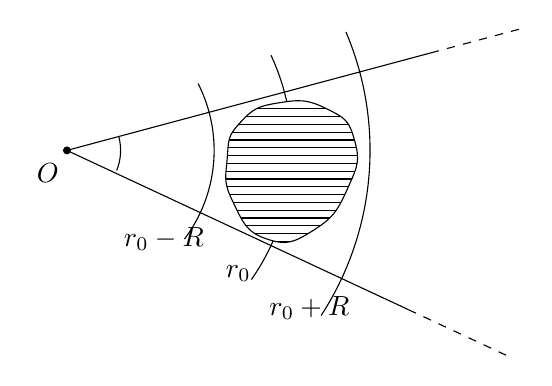
\begin{tikzpicture}[>=stealth,scale=1.1]
  \fill (0,0) circle (1.3pt);
  \node at (-0.22,-0.26) {$O$};
  \draw (-22:0.62) arc (-22:15:0.62);
  \draw (0,0) -- (15:4.35);
  \draw[dashed] (15:4.35) -- (15:5.45);
  \draw (0,0) -- (-25:4.35);
  \draw[dashed] (-25:4.35) -- (-25:5.65);
  \draw (27:1.7) arc (27:-37:1.7);
  \draw (25:2.6) arc (25:-35:2.6);
  \draw (23:3.5) arc (23:-33:3.5);
  \begin{scope}
    \clip plot[smooth cycle,tension=0.9] coordinates
      {(1.85,-0.1) (2.0,0.32) (2.45,0.55) (3.0,0.48) (3.32,0.12)
       (3.25,-0.42) (2.85,-0.92) (2.3,-1.02) (1.92,-0.6)};
    \fill[white] (1.6,-1.2) rectangle (3.6,0.8);
    \foreach \y in {-1.05,-0.96,...,0.55} \draw (1.6,\y) -- (3.6,\y);
  \end{scope}
  \draw plot[smooth cycle,tension=0.9] coordinates
    {(1.85,-0.1) (2.0,0.32) (2.45,0.55) (3.0,0.48) (3.32,0.12)
     (3.25,-0.42) (2.85,-0.92) (2.3,-1.02) (1.92,-0.6)};
  \node at (1.12,-1.02) {$r_{0}-R$};
  \node at (1.98,-1.42) {$r_{0}$};
  \node at (2.80,-1.82) {$r_{0}+R$};
\end{tikzpicture}

图 A4.1
\end{minipage}

当 $r_{0}=|z|\to\infty$ 时我们看到 $\sigma\to0$。更精确地，对大的 $|z|$ 有
\[
0\ \leq\ \sigma\ \leq\ \frac{4R}{|z|}\,.
\]
对足够大的 $|z|$，这意味着
\begin{align*}
|(Au)(z)|\ &\leq\ \frac{1}{2\pi}\ \int_{\operatorname{supp}(v)}\ |v(r,\theta)|\,dr\,d\theta\\
&\leq\ \frac{1}{2\pi}\ \int_{|z|-R}^{|z|+R}\ \Bigl(\int_{\Gamma}\ \|u\|_{\infty}\,d\theta\Bigr)\,dr\,,
\end{align*}
其中 $\Gamma$ 是一个开集，其测度 $(\Gamma)\leq\sigma$。于是
\begin{align*}
|(Au)(z)|\ &\leq\ \tfrac{1}{2\pi}\,2R\,\|u\|_{\infty}\,\sigma\\
&\leq\ \tfrac{4R^{2}}{\pi}\,\|u\|_{\infty}\,\tfrac{1}{|z|}\\
&\leq\ \operatorname{const}\,(u)\,\tfrac{1}{|z|}
\end{align*}
对足够大的 $|z|$ 成立。
\end{proof}

我们将利用这个命题把映射 $A$ 延拓到球面上，并接着研究%
\trRiemann\trSphere{} $S^{2}=\C\cup\{\infty\}$ 上的\trCauchy-\trRiemann%
\trOperator。我们通过定义如下两个\trChart{}赋予 $S^{2}$ 复\trManifold{}结构：
\begin{equation}\label{eq:sphere-charts}
\begin{aligned}
U\ &=\ \C\ \xrightarrow{\ \alpha\ }\ \C\ :\ z\ \longmapsto\ z\\
V\ &=\ \bigl(\C\setminus\{0\}\bigr)\cup\{+\infty\}\ \xrightarrow{\ \beta\ }\ \C\ :\ z\ \longmapsto
\begin{cases}
\dfrac{1}{z} & \text{若 }\ z\ \neq\ \infty\\[6pt]
0 & \text{若 }\ z\ =\ \infty\,.
\end{cases}
\end{aligned}
\end{equation}
显然 $\alpha$ 与 $\beta$ 都是\trHomeomorphism{}\footnote{原书 \eqref{eq:sphere-charts} 中 $\beta$ 之分段定义及下文转移映射均多排 bar（印作 $\tfrac{1}{\bar{z}}$）——下文明书 $u\bigl(\tfrac{1}{z}\bigr)=u\circ\beta^{-1}(z)$ 且全纯唯 $\tfrac{1}{z}$ 成立，均径改作 $\tfrac{1}{z}$。——译者注}，而 $\alpha\circ\beta^{-1}:%
\beta(U\cap V)\to\alpha(U\cap V)$ 是映射 $z\mapsto\frac{1}{z}$，从而是%
\trHolomorphic{}的。于是我们在 $S^{2}$ 上有一个自然的%
\trComplexStructure，记作 $i$。现在考虑\trVectorBundle
\[
\begin{aligned}
S^{2}\times\C^{n}\ &\longrightarrow\ S^{2}\\
X\ &\longrightarrow\ S^{2}\,,
\end{aligned}
\]
其位于 $z\in S^{2}$ 之上的\trFiber{} $X_{z}$ 由一切复反线性映射%
 $\varphi:T_{z}S^{2}\to\C^{n}$ 组成。为了在这些丛的 $C^{\infty}$-\trSection{}%
上定义\trCauchy-\trRiemann\trOperator{} $\bar{\partial}$，我们把 $S^{2}\times%
\C^{n}\to S^{2}$ 的\trSmooth\trSection{}之空间记作 $C^{\infty}(S^{2}\times\C^{n})$，%
即 $C^{\infty}(S^{2}\times\C^{n})=C^{\infty}(S^{2},\C^{n})$，而把 $X\to S^{2}$ %
的\trSmooth\trSection{}之空间记作 $C^{\infty}(X)$。我们定义%
 $\bar{\partial}:C^{\infty}(S^{2}\times\C^{n})\to C^{\infty}(X)$ 为
\begin{equation}\label{eq:cr-section-def}
(\bar{\partial}u)(z)\ =\ Tu(z)\ +\ i\,Tu(z)\,i\,,
\end{equation}
其中 $Tu(z):T_{z}S^{2}\to\C^{n}$（$z\in S^{2}$）是 $u$ 的切映射\footnote{原书 \eqref{eq:cr-section-def} 之左端印作「$(\bar{\partial}f)(z)$」，与下文「$u$ 之切映射」混称，其 $f$ 系 $u$ 之误，此处径改。——译者注}。注意
\[
(\bar{\partial}u)(z)\circ i\ =\ -i\circ(\bar{\partial}u)(z)\,,
\]
故 $\bar{\partial}$ 确实是良定义的。

现设 $g\in C^{\infty}(X)$。利用一个从属于我们这个特定的\trAtlas{}~%
\eqref{eq:sphere-charts} 的\trPartitionOfUnity{}，%
我们有分解
\[
g\ =\ g_{U}\ +\ g_{V}\,,
\]
其中 $\operatorname{supp}(g_{U})\subset U$，$\operatorname{supp}(g_{V})\subset V$。%
映射 $g_{U}(z):\C\to\C^{n}$ 对每个 $z\in U=\C$ 都是复反线性的，并且关于 $z$ %
具有\trCompactSupport。于是
\[
z\ \longmapsto\ g_{U}(z)(1)
\]
属于 $\mathcal{D}$。我们可以解出满足
\[
u_{s}+iu_{t}\ =\ g_{U}(\cdot)(1)\ =:\ \hat{g}_{U}\ \in\ C^{\infty}(\C,\C^{n})
\]
的 $u\in C^{\infty}(\C,\C^{n})$\footnote{原书此两式均印作 $g_{V}(\cdot)(1)=:\hat{g}_{V}$ 与 $u=A\hat{g}_{V}$，其 $V$ 系 $U$ 之误（上下文皆 $g_{U}$，结论 $\bar{\partial}u=g_{U}$ 于 $U=\C$），两处均径改。——译者注}，即取
\[
u\ =\ A\hat{g}_{U}\,.
\]
我们观察到
\begin{align*}
(\bar{\partial}u)(z)(1)\ &=\ \Bigl[\bigl(Tu(z)\ +\ i\,Tu(z)\,i\bigr)\Bigr](1)\\
&=\ u_{s}(z)\ +\ i\,u_{t}(z)\\
&=\ g_{U}(z)(1)\,.
\end{align*}
由于 $\bar{\partial}u(z)$ 是反线性的，在 $U=\C$ 上我们有 $\bar{\partial}u=g_{U}$。%
据\cref{prop:au-decay-at-infinity}，当 $|z|\to\infty$ 时 $u(z)\to0$；此外，%
$\bar{\partial}u(z)=0$ 在 $\hat{g}_{U}$ 的支撑之外成立，故 $u$ 在 $|z|$ 大时是%
\trHolomorphic{}的。考虑 $V\setminus\{\infty\}$ 上的映射
\[
\C\setminus\{0\}\ \longrightarrow\ \C^{n}\ :\ z\ \longmapsto\ u\Bigl(\frac{1}{z}\Bigr)\ =\ u\circ\beta^{-1}(z)\,.
\]
这个映射在 $0$ 的一个去心\trNeighborhood{}内是\trHolomorphic{}的，并且当%
 $z\to0$ 时 $u\bigl(\frac{1}{z}\bigr)\to0$。于是，由单复变理论中众所周知的%
经典结果，$0$ 是一个\trRemovableSingularity。因此，可以把 $u$ 视为 $S^{2}$ 上一个%
在 $\infty$ 处为零的\trSmooth{}函数。由\cref{prop:au-decay-at-infinity}我们%
特别得出

\begin{proposition}\label{prop:extend-a-to-sphere}
映射 $A$ 定义了一个从 $\mathcal{D}$ 到子空间 $\bigl\{f\in C^{\infty}(S^{2},\C^{n})\ \bigm|\ f(\infty)=0\bigr\}\subset C^{\infty}(S^{2},\C^{n})$ 的\trLinearOperator，%
且满足
\[
\bar{\partial}\circ A\ =\ \mathrm{Id}\,.
\]
\end{proposition}

回到我们先前的讨论：我们已经求得解方程 $\bar{\partial}u=g_{U}$ 的%
 $u\in C^{\infty}(S^{2}\times\C^{n})$；由于 $S^{2}\setminus\{0\}$ 双%
\trHolomorphic{}于 $\C$，用同样的论证我们求得满足 $\bar{\partial}v=g_{V}$ 的%
 $v\in C^{\infty}(S^{2}\times\C^{n})$\footnote{原书此句印作「the $g_{V}$ satisfying …」，其 $g_{V}$ 系 $v$ 之误（$g_{V}$ 已由单位分解给出，所求者为 $v$），此处径改。——译者注}。于是 $\bar{\partial}(u+v)=g_{U}+g_{V}=g$，%
这证明 $\bar{\partial}$ 是满射的。另一方面，若 $\bar{\partial}u=0$，我们便%
得到一个\trBounded{}的\trHolomorphic{}函数 $u:\C\to\C^{n}$，它由%
\trLiouville{}定理是一个常值映射。总括起来，我们证明了

\begin{theorem}\label{thm:cr-sphere-surjective}
映射 $\bar{\partial}:C^{\infty}(S^{2}\times\C^{n})\to C^{\infty}(X)$ 是一个%
满射的\trLinearOperator，其\trKernel{}由全体常值映射组成。作为实（相应地，%
复）线性算子，其\trKernel{}的维数为 $2n$（相应地，$n$）。
\end{theorem}

接下来我们想把 $\bar{\partial}$ 当作基于 $L^{p}$-空间（$1<p<\infty$）的%
\trSobolev{}空间框架中的一个算子来研究。我们从下述出自\trDouglis{}与%
\trNirenberg{} [63] 的估计开始。把 $\mathcal{D}$ 中支撑含于\trUnitBall{}的%
函数所成的子空间记作 $\mathcal{D}_{1}$。我们把由下式定义的%
\trNorm{}写作 $|\cdot|_{k,p}$：
\[
|u|_{k,p}^{p}\ =\ \sum_{|\alpha|\leq k}\ \bigl|D^{\alpha}u\bigr|_{L^{p}(B_{1}(0))}^{p}\,.
\]
此处 $k\in\mathbb{N}$ 而 $1<p<\infty$。[63] 中给出的基本估计即是下述

\begin{theorem}\label{thm:douglis-nirenberg}
对给定的 $k\in\mathbb{N}$ 与 $1<p<\infty$，存在正常数 $c=c(k,p)$，使得
\[
|\bar{\partial}u|_{k,p}\ \geq\ c\,|u|_{k+1,p}
\]
对一切 $u\in\mathcal{D}_{1}$ 成立。
\end{theorem}

为了给截面映射 $\bar{\partial}:C^{\infty}(S^{2}\times\C^{n})\to C^{\infty}(X)$ %
求得一些\trSobolev{}型估计，我们取 $S^{2}$ 的一个有限覆盖 $U_{1},\ldots,U_{m}$，%
使得诸 $U_{j}$ 都双\trHolomorphic{}于 $0$ 附近的开单位\trDisc{} $B$。令%
 $\beta_{1},\ldots,\beta_{m}$ 是从属于它的一个\trPartitionOfUnity{}\footnote{原书印作「$\beta_{1},\ldots,\beta_{n}$」，其下标 $n$ 系 $m$ 之误（所从属之覆盖与下文求和均作 $m$），此处径改。——译者注}。记 $\varphi_{j}:U_{j}\to B$ %
为适宜的双\trHolomorphic{}\trDiffeomorphism，我们对 $k\in\mathbb{N}$、%
 $1<p<\infty$ 定义\trNorm{} $\|\cdot\|_{k,p}$ 为
\[
\|u\|_{k,p}^{p}\ =\ \sum_{j=1}^{m}\ \Bigl|(\beta_{j}\circ\varphi_{j}^{-1})(u\circ\varphi_{j}^{-1})\Bigr|_{k,p}^{p}\,.
\]
容易证明，由此程序得到的 $C^{\infty}(S^{2}\times\C^{n})$ 上的所有\trNorm{}都是%
等价的。对丛 $X\to S^{2}$，我们取覆盖 $\varphi_{j}$ 的光滑复线性%
\trTrivialization{} $\psi_{j}:X|_{U_{j}}\to B\times\C^{n}$。这就是说，下面的%
图是交换的：

\begin{center}
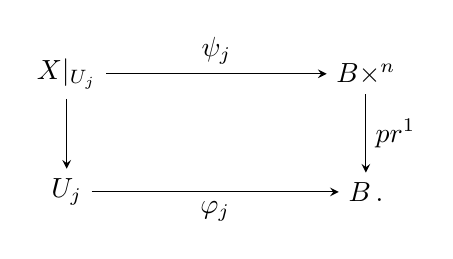
\begin{tikzpicture}[>=stealth]
  \node (x) at (0,1.5) {$X|_{U_{j}}$};
  \node (b) at (3.8,1.5) {$B\times\C^{n}$};
  \node (u) at (0,0) {$U_{j}$};
  \node (bb) at (3.8,0) {$B\,.$};
  \draw[->] (x) -- node[above]{$\psi_{j}$} (b);
  \draw[->] (x) -- (u);
  \draw[->] (b) -- node[right]{$pr^{1}$} (bb);
  \draw[->] (u) -- node[below]{$\varphi_{j}$} (bb);
\end{tikzpicture}
\end{center}

若 $f$ 是 $X$ 的一个\trSection，我们定义\trNorm{} $\vert\vert\vert f\vert\vert\vert_{k,p}$ %
为
\[
\vert\vert\vert f\vert\vert\vert_{k,p}^{p}\ =\ \sum_{j=1}^{m}\ \Bigl|\psi_{j}\bigl(\varphi_{j}^{-1}\bigr)\Bigl((\beta_{j}\circ\varphi_{j}^{-1})(f\circ\varphi_{j}^{-1})\Bigr)\Bigr|_{k,p}^{p}\,.
\]
照此方式得到的所有\trNorm{}仍是等价的。我们简记 $\hat{\psi}_{j}=\psi_{j}(\varphi_{j}^{-1})$ %
与 $\hat{\beta}_{j}=\beta_{j}\circ\varphi_{j}^{-1}$。于是
\begin{align*}
&\hat{\psi}_{j}(z)\Bigl(\hat{\beta}_{j}(z)(\bar{\partial}u)\bigl(\varphi_{j}^{-1}(z)\bigr)\Bigr)\\
&\qquad=\ \hat{\beta}_{j}(z)\hat{\psi}_{j}(z)\Bigl((Tu)\bigl(\varphi_{j}^{-1}(z)\bigr)\ +\ i\,(Tu)\bigl(\varphi_{j}^{-1}(z)\bigr)i\Bigr)\\
&\qquad=\ \hat{\beta}_{j}(z)\hat{\psi}_{j}(z)\Bigl[\bigl(T(u\circ\varphi_{j}^{-1})(z)\ +\ i\,\bigl(T(u\circ\varphi_{j}^{-1})(z)\bigr)i\bigr)T\varphi_{j}\bigl(\varphi_{j}^{-1}(z)\bigr)\Bigr]\\
&\qquad=\ \hat{\beta}_{j}(z)\hat{\psi}_{j}(z)\Bigl[\bigl(T\hat{u}_{j}(z)\ +\ i\,T\hat{u}_{j}(z)i\bigr)T\varphi_{j}\bigl(\varphi_{j}^{-1}(z)\bigr)\Bigr]\,,
\end{align*}
其中 $\hat{u}_{j}=u\circ\varphi_{j}^{-1}$\footnote{原书印作「$\hat{u}_{j}=u_{j}\circ\varphi_{j}^{-1}$」，其 $u_{j}$ 无定义，系 $u$ 之漏排，径改；上行链第三式原书缺一右括号、第四式右括号错位（其 $i$ 误置于右括号之外，印作 $\bigl(T\hat{u}_{j}(z)+iT\hat{u}_{j}(z)\bigr)iT\varphi_{j}(z)$），径正；又上行链第三、四式之末因子原书均印作 $T\varphi_{j}(z)$，其 $z\in B$ 而 $\varphi_{j}$ 定义于 $U_{j}$，于 $z$ 处无定义，应为 $T\varphi_{j}\bigl(\varphi_{j}^{-1}(z)\bigr)$，径正。——译者注}。这立即给出估计
\[
\Bigl|\hat{\psi}_{j}\Bigl(\hat{\beta}_{j}(\bar{\partial}u)\bigl(\varphi_{j}^{-1}\bigr)\Bigr)\Bigr|_{0,p}^{p}\ \geq\ d_{j}^{p}\,\Bigl|\hat{\beta}_{j}\Bigl(\frac{\partial}{\partial s}+i\frac{\partial}{\partial t}\Bigr)\hat{u}_{j}\Bigr|_{0,p}^{p}\,,
\]
其中常数 $d_{j}$ 适宜且与 $u$ 无关。若 $d=\inf\{d_{1},\ldots,d_{m}\}$，则
\begin{align*}
\vert\vert\vert\bar{\partial}u\vert\vert\vert_{0,p}\ &\geq\ d\,\Bigl(\sum_{j=1}^{m}\ \Bigl|\hat{\beta}_{j}\Bigl(\frac{\partial}{\partial s}+i\frac{\partial}{\partial t}\Bigr)\hat{u}_{j}\Bigr|_{0,p}^{p}\Bigr)^{1/p}\\
&=\ d\,\Bigl(\sum_{j=1}^{m}\ \Bigl|\Bigl(\frac{\partial}{\partial s}+i\frac{\partial}{\partial t}\Bigr)(\hat{\beta}_{j}\hat{u}_{j})\ -\ \Bigl(\Bigl(\frac{\partial}{\partial s}+i\frac{\partial}{\partial t}\Bigr)\hat{\beta}_{j}\Bigr)\hat{u}_{j}\Bigr|_{0,p}^{p}\Bigr)^{1/p}\\
&\geq\ d\,\Bigl(\sum_{j=1}^{m}\ \Bigl|\Bigl(\frac{\partial}{\partial s}+i\frac{\partial}{\partial t}\Bigr)(\hat{\beta}_{j}\hat{u}_{j})\Bigr|_{0,p}^{p}\Bigr)^{1/p}\ -\ a\,\Bigl(\sum_{j=1}^{m}\ \bigl|\chi_{j}\hat{u}_{j}\bigr|_{0,p}^{p}\Bigr)^{1/p}
\end{align*}
对某个与 $u$ 的选取无关的适宜常数 $a>0$ 成立。此处 $\chi_{j}$ 是 $\hat{\beta}_{j}$ %
之支撑的示性函数。于是，应用\cref{thm:douglis-nirenberg}得
\begin{align*}
\vert\vert\vert\bar{\partial}u\vert\vert\vert_{0,p}\ &\geq\ d\,\Bigl(\sum_{j=1}^{m}\ c^{p}\,\bigl|\hat{\beta}_{j}\hat{u}_{j}\bigr|_{1,p}^{p}\Bigr)^{1/p}\ -\ a\,\Bigl(\sum_{j=1}^{m}\ \bigl|\chi_{j}\hat{u}_{j}\bigr|_{0,p}^{p}\Bigr)^{1/p}\\
&\geq\ c'\,\vert\vert\vert u\vert\vert\vert_{1,p}\ -\ a'\,\vert\vert\vert u\vert\vert\vert_{0,p}
\end{align*}
其中常数 $a'$、$c'>0$ 适宜且与 $u$ 无关。我们证明了

\begin{theorem}\label{thm:cr-lp-estimate}
存在常数 $a$、$c>0$，使得对一切 $u\in C^{\infty}(S^{2}\times\C^{n})$ 有
\[
\vert\vert\vert\bar{\partial}u\vert\vert\vert_{0,p}\ \geq\ c\,\vert\vert\vert u\vert\vert\vert_{1,p}\ -\ a\,\vert\vert\vert u\vert\vert\vert_{0,p}\,.
\]
\end{theorem}

把 $W^{1,p}(S^{2}\times\C^{n})$ 与 $L^{p}(X)$ 定义为空间 $C^{\infty}(S^{2}\times\C^{n})$ %
与 $C^{\infty}(X)$ 分别关于\trNorm{} $\vert\vert\vert\cdot\vert\vert\vert_{1,p}$ 与%
 $\vert\vert\vert\cdot\vert\vert\vert_{0,p}$ 的\trCompletion。由 $W^{1,p}\hookrightarrow L^{p}$ %
的紧\trEmbedding{}并据\cref{thm:cr-lp-estimate}，我们得知 $\bar{\partial}:W^{1,p}(S^{2}\times\C^{n})\to L^{p}(X)$ %
具有\trClosed\trRange。又据\cref{thm:cr-sphere-surjective}，其\trRange{}含有%
\trDense{}集 $C^{\infty}(X)$，故我们推出 $\bar{\partial}\bigl(W^{1,p}(S^{2}\times\C^{n})\bigr)=L^{p}(X)$，%
从而 $\bar{\partial}$ 是满射的。

另一方面，由内部椭圆\trRegularity{}理论，或者由「\trHolomorphic{}的%
\trDistribution{}必是\trHolomorphic{}函数」这一众所周知%
的事实，从 $\bar{\partial}u=0$ 我们得出：$u$ 是\trHolomorphic{}且\trBounded{} %
的，从而必为常值。

我们证明了

\begin{theorem}\label{thm:cr-fredholm-w1p}
算子 $\bar{\partial}:W^{1,p}(S^{2}\times\C^{n})\to L^{p}(X)$ 是一个满射的%
\trFredholm{}算子，其\trKernel{}由常值函数组成。于是，把 $\bar{\partial}$ %
视为实算子时其指标为 $2n$。
\end{theorem}

稍加更多的努力并借助初等的泛函分析，还可以证明

\begin{theorem}\label{thm:cr-higher-estimate}
对每个 $k\in\mathbb{N}$ 与 $1<p<\infty$，存在正常数 $c=c(k,p)$ 与 $a=a(k,p)$，%
使得
\[
\vert\vert\vert\bar{\partial}u\vert\vert\vert_{k,p}\ \geq\ c\,\vert\vert\vert u\vert\vert\vert_{k+1,p}\ -\ a\,\vert\vert\vert u\vert\vert\vert_{0,p}\,,
\]
对一切 $u\in C^{\infty}(S^{2}\times\C^{n})$ 成立。
\end{theorem}

作为从 $W^{k+1,p}(S^{2}\times\C^{n})$ 到 $W^{k,p}(X)$ 的算子，线性算子%
 $\bar{\partial}$ 仍是一个满射的\trFredholm{}算子，其\trKernel{}由常值函数%
组成。关于一阶椭圆\trDifferentialEquation{}组的一般处理，我们请读者查阅%
\trVekua{}的书 [215] 或其英译本。
